% Options for packages loaded elsewhere
\PassOptionsToPackage{unicode}{hyperref}
\PassOptionsToPackage{hyphens}{url}
%
\documentclass[
  ignorenonframetext,
]{beamer}
\usepackage{pgfpages}
\setbeamertemplate{caption}[numbered]
\setbeamertemplate{caption label separator}{: }
\setbeamercolor{caption name}{fg=normal text.fg}
\beamertemplatenavigationsymbolsempty
% Prevent slide breaks in the middle of a paragraph
\widowpenalties 1 10000
\raggedbottom
\setbeamertemplate{part page}{
  \centering
  \begin{beamercolorbox}[sep=16pt,center]{part title}
    \usebeamerfont{part title}\insertpart\par
  \end{beamercolorbox}
}
\setbeamertemplate{section page}{
  \centering
  \begin{beamercolorbox}[sep=12pt,center]{part title}
    \usebeamerfont{section title}\insertsection\par
  \end{beamercolorbox}
}
\setbeamertemplate{subsection page}{
  \centering
  \begin{beamercolorbox}[sep=8pt,center]{part title}
    \usebeamerfont{subsection title}\insertsubsection\par
  \end{beamercolorbox}
}
\AtBeginPart{
  \frame{\partpage}
}
\AtBeginSection{
  \ifbibliography
  \else
    \frame{\sectionpage}
  \fi
}
\AtBeginSubsection{
  \frame{\subsectionpage}
}
\usepackage{amsmath,amssymb}
\usepackage{lmodern}
\usepackage{iftex}
\ifPDFTeX
  \usepackage[T1]{fontenc}
  \usepackage[utf8]{inputenc}
  \usepackage{textcomp} % provide euro and other symbols
\else % if luatex or xetex
  \usepackage{unicode-math}
  \defaultfontfeatures{Scale=MatchLowercase}
  \defaultfontfeatures[\rmfamily]{Ligatures=TeX,Scale=1}
\fi
% Use upquote if available, for straight quotes in verbatim environments
\IfFileExists{upquote.sty}{\usepackage{upquote}}{}
\IfFileExists{microtype.sty}{% use microtype if available
  \usepackage[]{microtype}
  \UseMicrotypeSet[protrusion]{basicmath} % disable protrusion for tt fonts
}{}
\makeatletter
\@ifundefined{KOMAClassName}{% if non-KOMA class
  \IfFileExists{parskip.sty}{%
    \usepackage{parskip}
  }{% else
    \setlength{\parindent}{0pt}
    \setlength{\parskip}{6pt plus 2pt minus 1pt}}
}{% if KOMA class
  \KOMAoptions{parskip=half}}
\makeatother
\usepackage{xcolor}
\newif\ifbibliography
\usepackage{longtable,booktabs,array}
\usepackage{calc} % for calculating minipage widths
\usepackage{caption}
% Make caption package work with longtable
\makeatletter
\def\fnum@table{\tablename~\thetable}
\makeatother
\usepackage{graphicx}
\makeatletter
\def\maxwidth{\ifdim\Gin@nat@width>\linewidth\linewidth\else\Gin@nat@width\fi}
\def\maxheight{\ifdim\Gin@nat@height>\textheight\textheight\else\Gin@nat@height\fi}
\makeatother
% Scale images if necessary, so that they will not overflow the page
% margins by default, and it is still possible to overwrite the defaults
% using explicit options in \includegraphics[width, height, ...]{}
\setkeys{Gin}{width=\maxwidth,height=\maxheight,keepaspectratio}
% Set default figure placement to htbp
\makeatletter
\def\fps@figure{htbp}
\makeatother
\setlength{\emergencystretch}{3em} % prevent overfull lines
\providecommand{\tightlist}{%
  \setlength{\itemsep}{0pt}\setlength{\parskip}{0pt}}
\setcounter{secnumdepth}{-\maxdimen} % remove section numbering
\ifLuaTeX
  \usepackage{selnolig}  % disable illegal ligatures
\fi
\IfFileExists{bookmark.sty}{\usepackage{bookmark}}{\usepackage{hyperref}}
\IfFileExists{xurl.sty}{\usepackage{xurl}}{} % add URL line breaks if available
\urlstyle{same} % disable monospaced font for URLs
\hypersetup{
  pdftitle={Group 11 Final Presentation},
  pdfauthor={Tom Tribe, Ken MacIver, Jundi Yang, Mei Huang},
  hidelinks,
  pdfcreator={LaTeX via pandoc}}

\title{Group 11 Final Presentation}
\author{Tom Tribe, Ken MacIver, Jundi Yang, Mei Huang}
\date{2022-10-11}

\begin{document}
\frame{\titlepage}

\begin{frame}{Group 11: Diamonds Dataset}
\protect\hypertarget{group-11-diamonds-dataset}{}
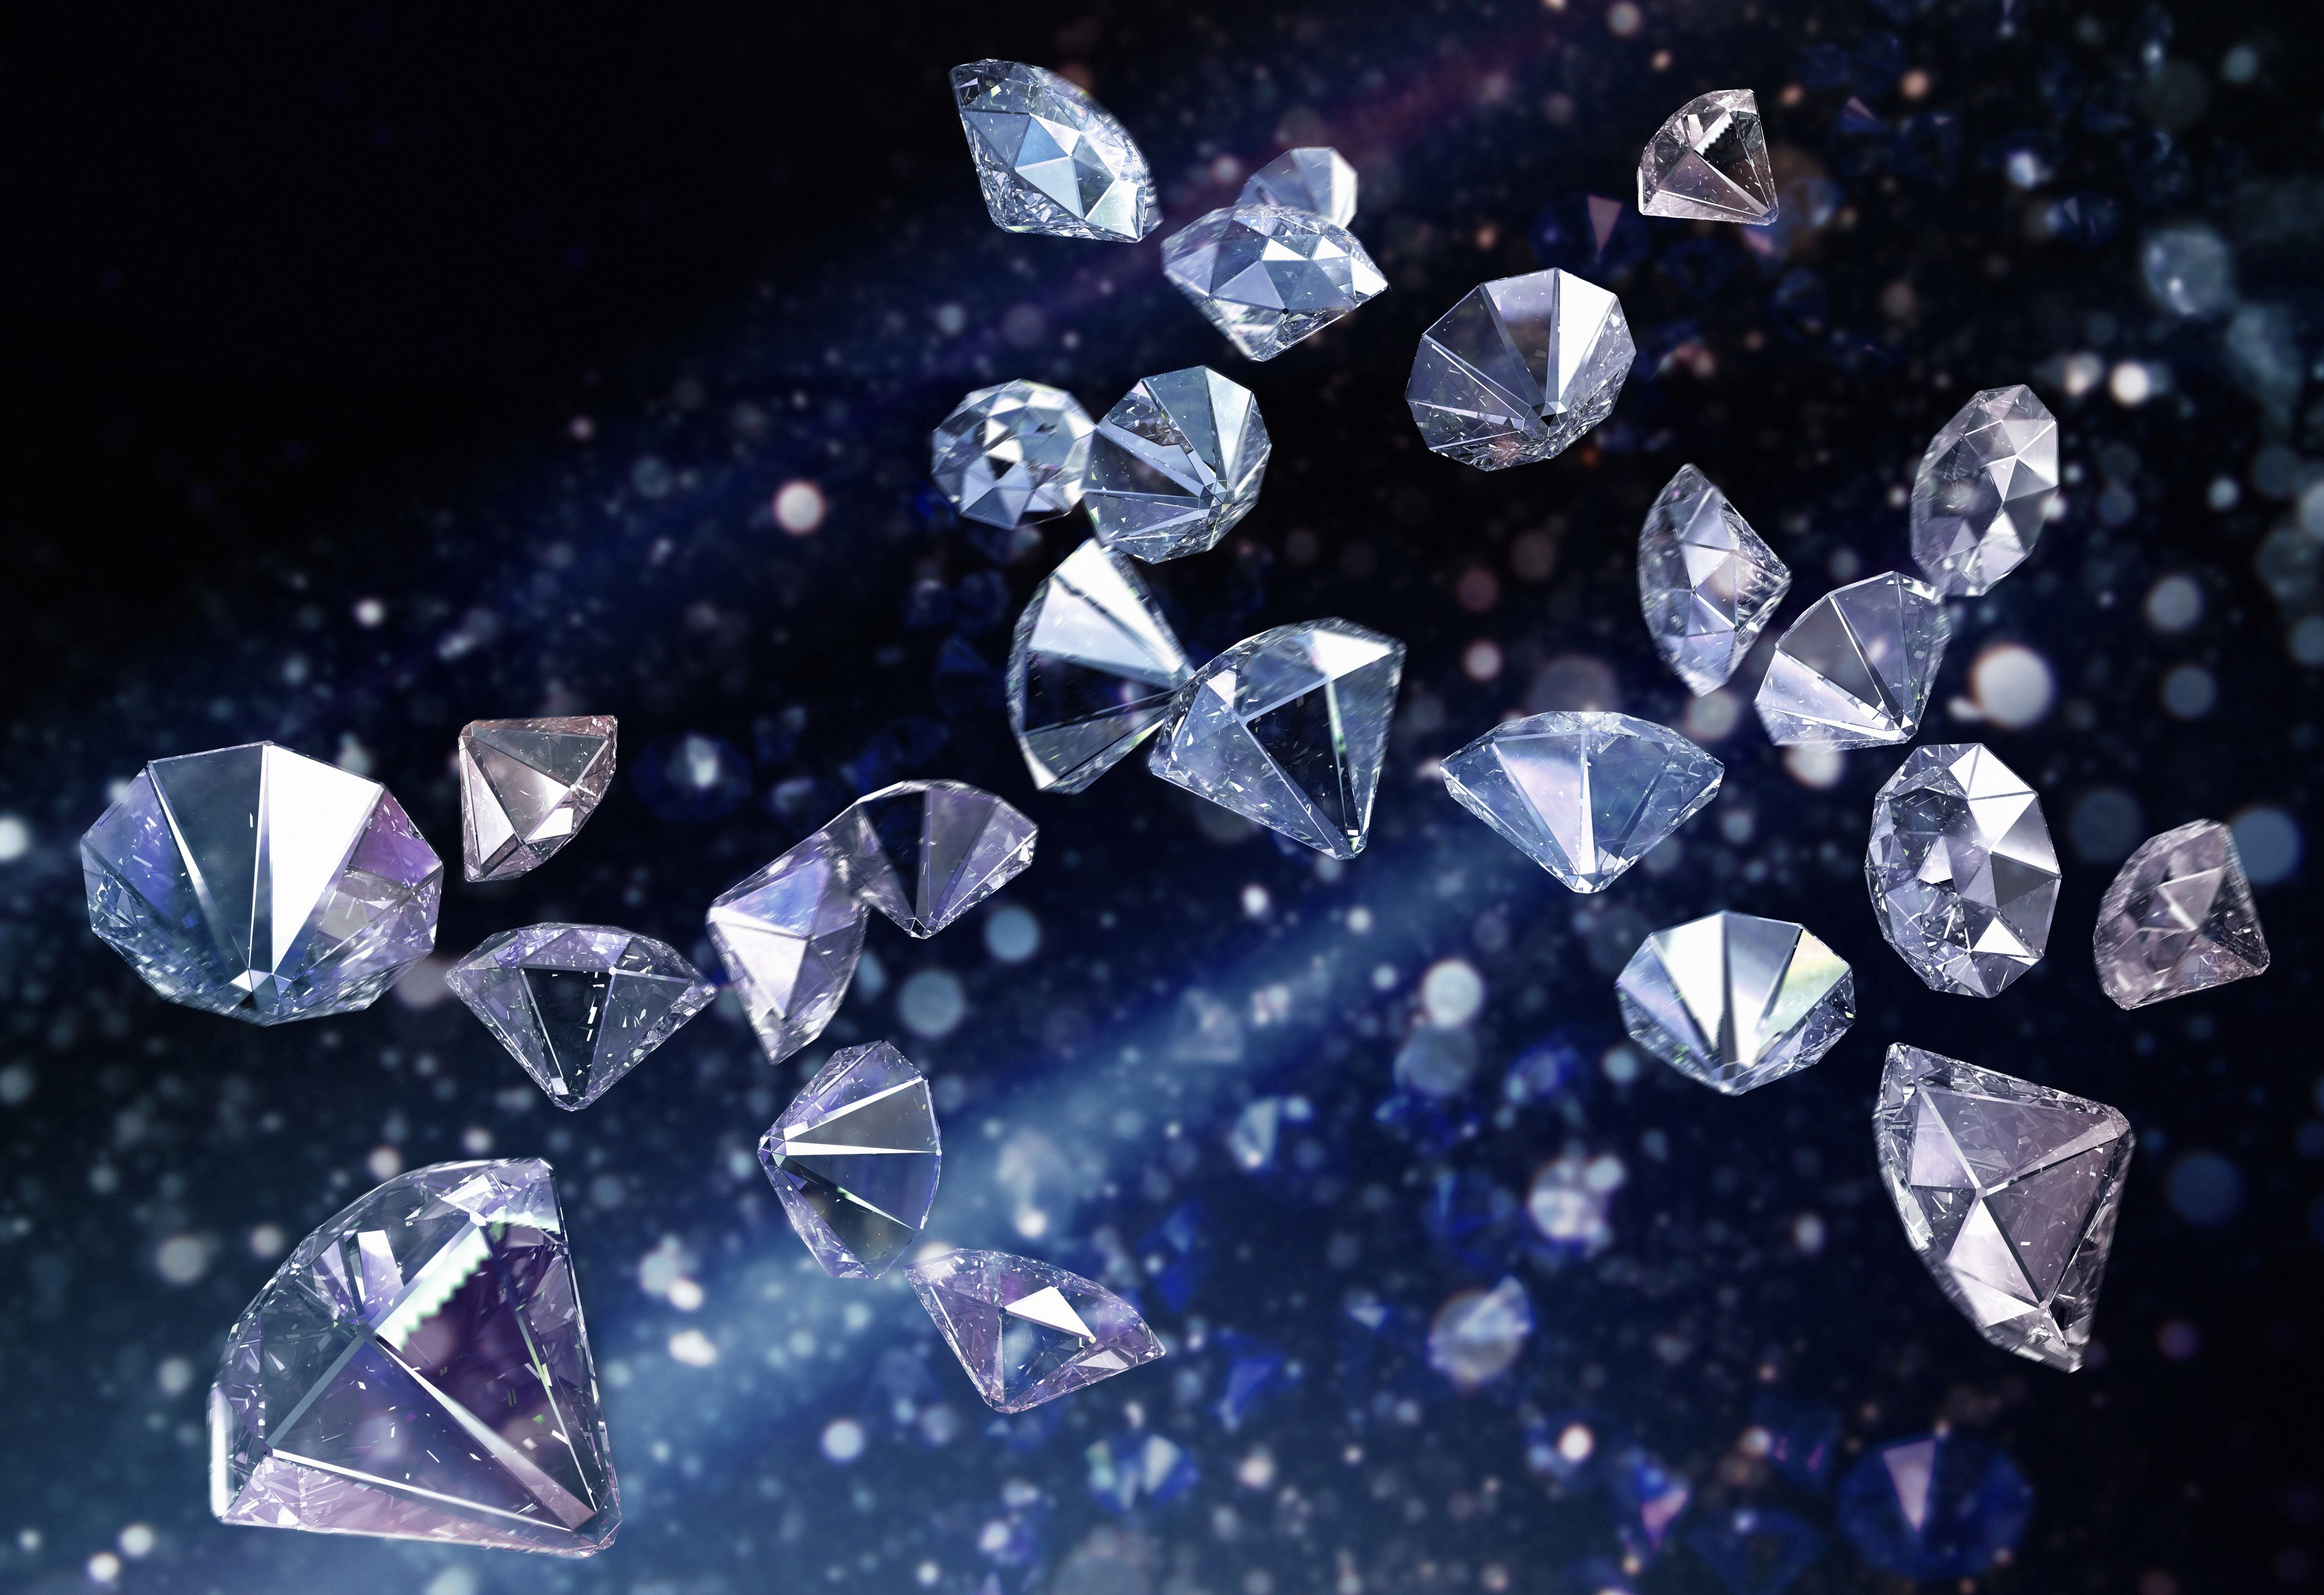
\includegraphics{./Diamonds.jpg}
\end{frame}

\begin{frame}{Group Members (photos)}
\protect\hypertarget{group-members-photos}{}
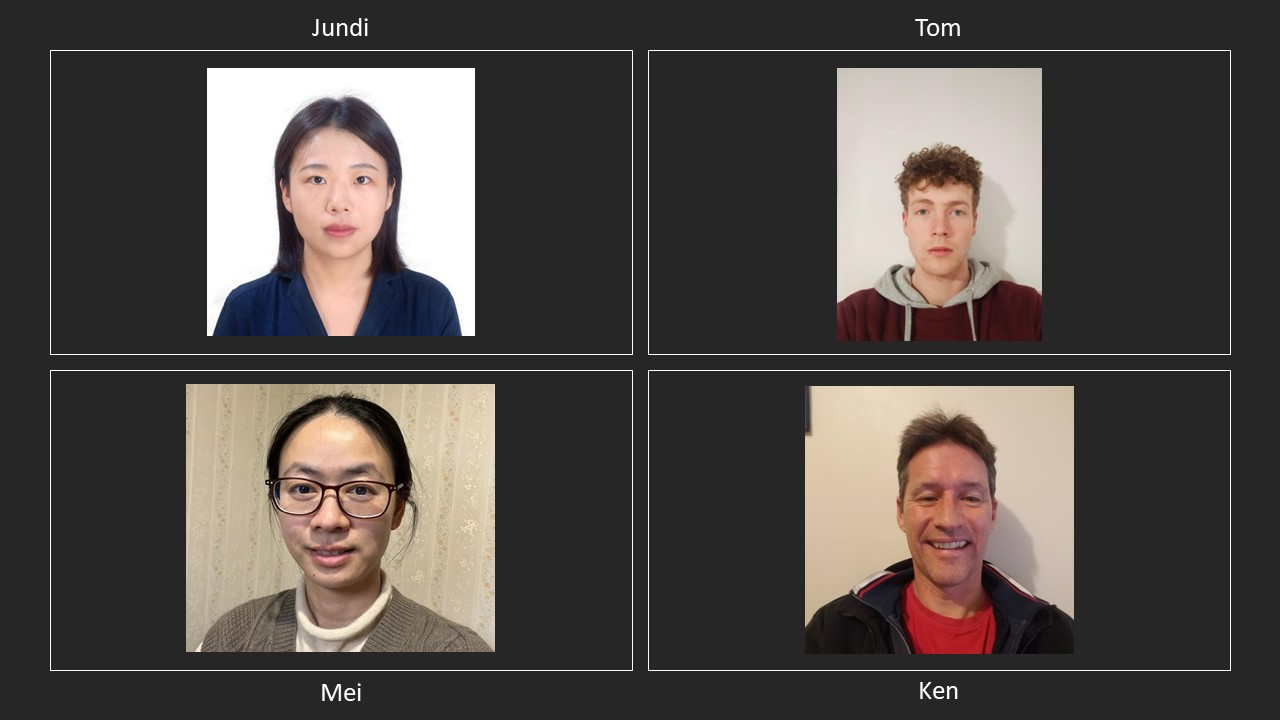
\includegraphics{./Photos3.jpg}
\end{frame}

\begin{frame}{Group Members (name, email, ORCID)}
\protect\hypertarget{group-members-name-email-orcid}{}
Tom Tribe

\begin{itemize}
\tightlist
\item
  \href{mailto:tom.tribe2016@gmail.com}{\nolinkurl{tom.tribe2016@gmail.com}}
\item
  0000-0002-5002-8066
\end{itemize}

Ken MacIver

\begin{itemize}
\tightlist
\item
  \href{mailto:ken.maciver68@gmail.com}{\nolinkurl{ken.maciver68@gmail.com}}
\item
  0000-0001-8999-4598
\end{itemize}

Jundi Yang

\begin{itemize}
\tightlist
\item
  \href{mailto:ivyli112358@gmail.com}{\nolinkurl{ivyli112358@gmail.com}}
\item
  0000-0003-0888-9564
\end{itemize}

Mei Huang

\begin{itemize}
\tightlist
\item
  \href{mailto:huangmei139@gmail.com}{\nolinkurl{huangmei139@gmail.com}}
\item
  0000-0003-2401-0679
\end{itemize}
\end{frame}

\begin{frame}{The Diamonds dataset}
\protect\hypertarget{the-diamonds-dataset}{}
\begin{itemize}
\tightlist
\item
  This large dataset has 53940 rows (diamonds) of ten variables (approx
  540,000 values)\linebreak 
\item
  Slow to process!\linebreak
\item
  There are seven numeric variables and three categorical
  variables\linebreak
\item
  We selected diamonds because it was conceptually simple to understand
  what each variable was measuring, and to have the opportunity to use
  the analytical techniques taught in STAT394 with a large
  dataset\linebreak
\end{itemize}
\end{frame}

\begin{frame}{The Variables}
\protect\hypertarget{the-variables}{}
\textcolor{red}{red font = categorical variable}

\begin{itemize}
\tightlist
\item
  carat: the diamond's weight
\item
  \textcolor{red}{cut: a measure of quality (4 levels)}
\item
  \textcolor{red}{color: a measure of colour quality (7 levels)}
\item
  \textcolor{red}{clarity: a measure of clearness (6 levels)}
\item
  x: length in mm
\item
  y: width in mm
\item
  z: depth in mm
\item
  depth: total depth percentage
\item
  table: width of top of diamond relative to widest point
\item
  price: the price of the diamond in US dollars
\end{itemize}

(List adapted from list at kaggle.com).
\end{frame}

\begin{frame}{Summary of Numeric Variables}
\protect\hypertarget{summary-of-numeric-variables}{}
\begin{longtable}[]{@{}
  >{\raggedright\arraybackslash}p{(\columnwidth - 14\tabcolsep) * \real{0.2317}}
  >{\raggedleft\arraybackslash}p{(\columnwidth - 14\tabcolsep) * \real{0.1098}}
  >{\raggedleft\arraybackslash}p{(\columnwidth - 14\tabcolsep) * \real{0.1098}}
  >{\raggedleft\arraybackslash}p{(\columnwidth - 14\tabcolsep) * \real{0.1098}}
  >{\raggedleft\arraybackslash}p{(\columnwidth - 14\tabcolsep) * \real{0.1098}}
  >{\raggedleft\arraybackslash}p{(\columnwidth - 14\tabcolsep) * \real{0.1098}}
  >{\raggedleft\arraybackslash}p{(\columnwidth - 14\tabcolsep) * \real{0.1098}}
  >{\raggedleft\arraybackslash}p{(\columnwidth - 14\tabcolsep) * \real{0.1098}}@{}}
\toprule()
\begin{minipage}[b]{\linewidth}\raggedright
\end{minipage} & \begin{minipage}[b]{\linewidth}\raggedleft
carat
\end{minipage} & \begin{minipage}[b]{\linewidth}\raggedleft
depth
\end{minipage} & \begin{minipage}[b]{\linewidth}\raggedleft
table
\end{minipage} & \begin{minipage}[b]{\linewidth}\raggedleft
price
\end{minipage} & \begin{minipage}[b]{\linewidth}\raggedleft
x
\end{minipage} & \begin{minipage}[b]{\linewidth}\raggedleft
y
\end{minipage} & \begin{minipage}[b]{\linewidth}\raggedleft
z
\end{minipage} \\
\midrule()
\endhead
sample size & 53940 & 53940 & 53940 & 53940 & 53940 & 53940 & 53940 \\
minimum & 0.20 & 43.00 & 43.00 & 326.00 & 0.00 & 0.00 & 0.00 \\
first quartile & 0.40 & 61.00 & 56.00 & 950.00 & 4.71 & 4.72 & 2.91 \\
median & 0.70 & 61.80 & 57.00 & 2401.00 & 5.70 & 5.71 & 3.53 \\
mean & 0.80 & 61.75 & 57.46 & 3932.80 & 5.73 & 5.73 & 3.54 \\
third quartile & 1.04 & 62.50 & 59.00 & 5324.25 & 6.54 & 6.54 & 4.04 \\
maximum & 5.01 & 79.00 & 95.00 & 18823.00 & 10.74 & 58.90 & 31.80 \\
IQR & 0.64 & 1.50 & 3.00 & 4374.25 & 1.83 & 1.82 & 1.13 \\
standard deviation & 0.47 & 1.43 & 2.23 & 3989.44 & 1.12 & 1.14 &
0.71 \\
skewness & 1.12 & -0.08 & 0.80 & 1.62 & 0.38 & 2.43 & 1.52 \\
kurtosis & 4.26 & 8.74 & 5.80 & 5.18 & 2.38 & 94.21 & 50.08 \\
\bottomrule()
\end{longtable}
\end{frame}

\begin{frame}{Cateogrical Summary}
\protect\hypertarget{cateogrical-summary}{}
\begin{table}[ht]
\centering
\begin{tabular}{rrrrrr}
  \hline
 Cut\vline & Fair & Good & Very Good & Premium & Ideal \\ 
  \hline
Count\vline & 1610 & 4960 & 12082 & 13791 & 21551\\
   \hline
\end{tabular}
\end{table}

\begin{table}[ht]
\centering
\begin{tabular}{rrrrrrrr}
  \hline
 Color\vline & J & I & H & G & F & E & D \\ 
  \hline
 Count\vline & 2808 & 5422 & 8304 & 11292 & 9542 & 9797 & 6775\\
   \hline
\end{tabular}
\end{table}

\begin{table}[ht]
\centering
\begin{tabular}{rrrrrrrrr}
  \hline
 Clarity\vline & I1 & SI2 & SI1 & VS2 & VS1 & VVS2 & VVS1 & IF \\ 
  \hline
  Count\vline & 741 & 9194 & 13065 & 12258 & 8171 & 5066 & 3655 & 1790\\
   \hline
\end{tabular}
\end{table}
\end{frame}

\begin{frame}{Pairs Plot}
\protect\hypertarget{pairs-plot}{}
\begin{figure}
\centering
\includegraphics{./pairs plot.jpg}
\caption{Pairs plot}
\end{figure}
\end{frame}

\begin{frame}{Normal QQ Plots}
\protect\hypertarget{normal-qq-plots}{}
\begin{figure}
\centering
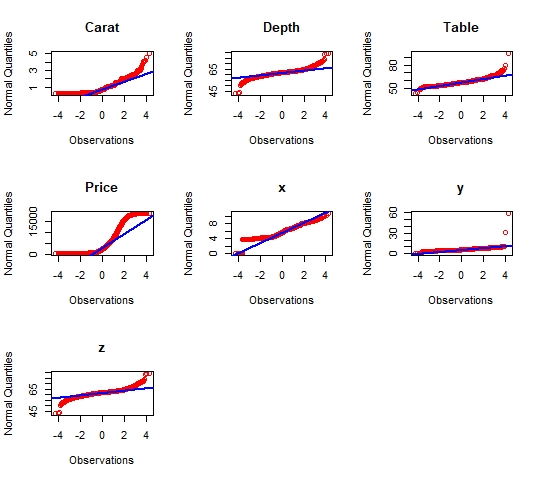
\includegraphics[width=\textwidth,height=0.85\textheight]{./Normal QQ Plots.jpeg}
\caption{Normal QQ Plots}
\end{figure}
\end{frame}

\begin{frame}{Correlation Plot}
\protect\hypertarget{correlation-plot}{}
\begin{figure}
\centering
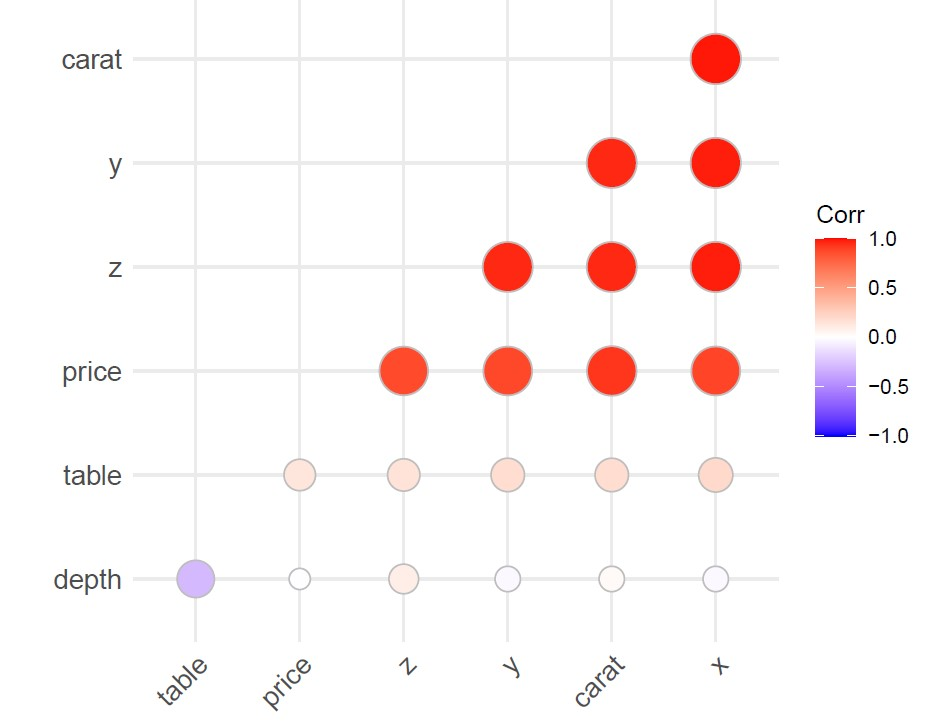
\includegraphics[width=\textwidth,height=0.85\textheight]{./Corrplot_diamonds.jpg}
\caption{Correlation Plot}
\end{figure}
\end{frame}

\begin{frame}{Price by Cateogrical}
\protect\hypertarget{price-by-cateogrical}{}
\begin{figure}
\centering
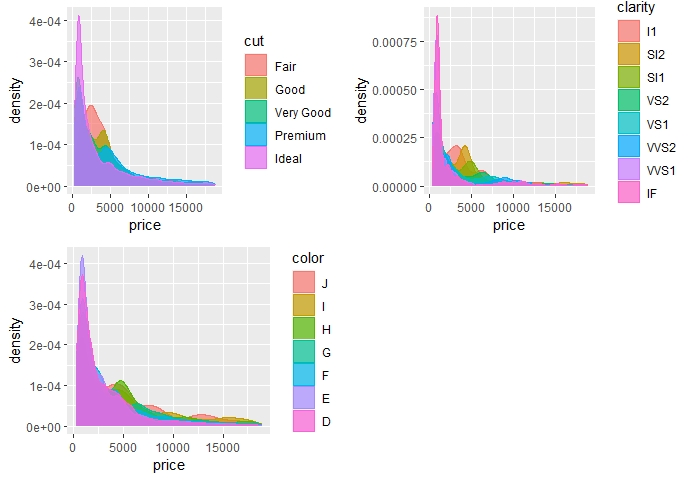
\includegraphics{./pricebycategorical.jpeg}
\caption{Price by Categorical}
\end{figure}
\end{frame}

\begin{frame}{Leading Question 1}
\protect\hypertarget{leading-question-1}{}
\begin{itemize}
\tightlist
\item
  How can we best predict diamond price using the other
  variables?\linebreak 
\item
  We intend to use the following techniques to investigate this
  question:\linebreak
\item
  Stepwise Regression, Principal Components Analysis, Principal
  Components Regression\linebreak
\end{itemize}
\end{frame}

\begin{frame}{Multiple Regression}
\protect\hypertarget{multiple-regression}{}
\begin{itemize}
\tightlist
\item
  Starting with the full model we used a stepwise regression procedure
  to find the best model for predicting diamond price.\linebreak
\item
  According to AIC the best model was:\linebreak
\item
  price \textasciitilde{} carat + cut + color + clarity + depth + table
  + x\linebreak 
\item
  All variables excluding y and z are significant in the model\linebreak
\item
  The `best' model had an Adjusted \(R^2\) of 91.98\%\linebreak 
\end{itemize}
\end{frame}

\begin{frame}{Regression Assumptions}
\protect\hypertarget{regression-assumptions}{}
\begin{figure}
\centering
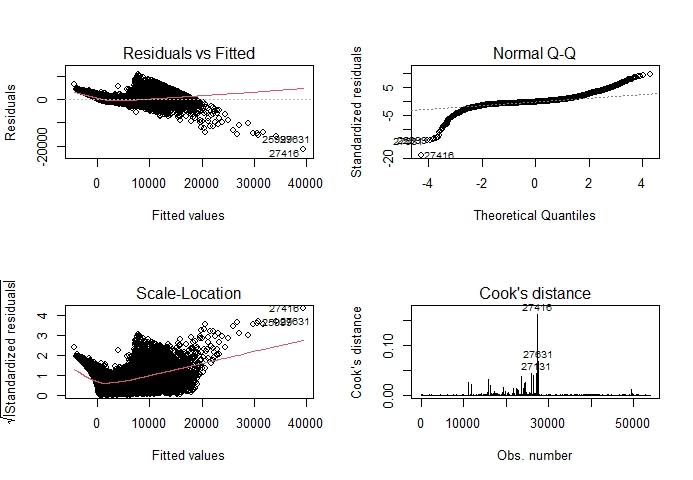
\includegraphics{./Regression Diagnostics.jpeg}
\caption{Regression Diagnostics}
\end{figure}
\end{frame}

\begin{frame}{Principal Components Analysis: Screeplot}
\protect\hypertarget{principal-components-analysis-screeplot}{}
\begin{figure}
\centering
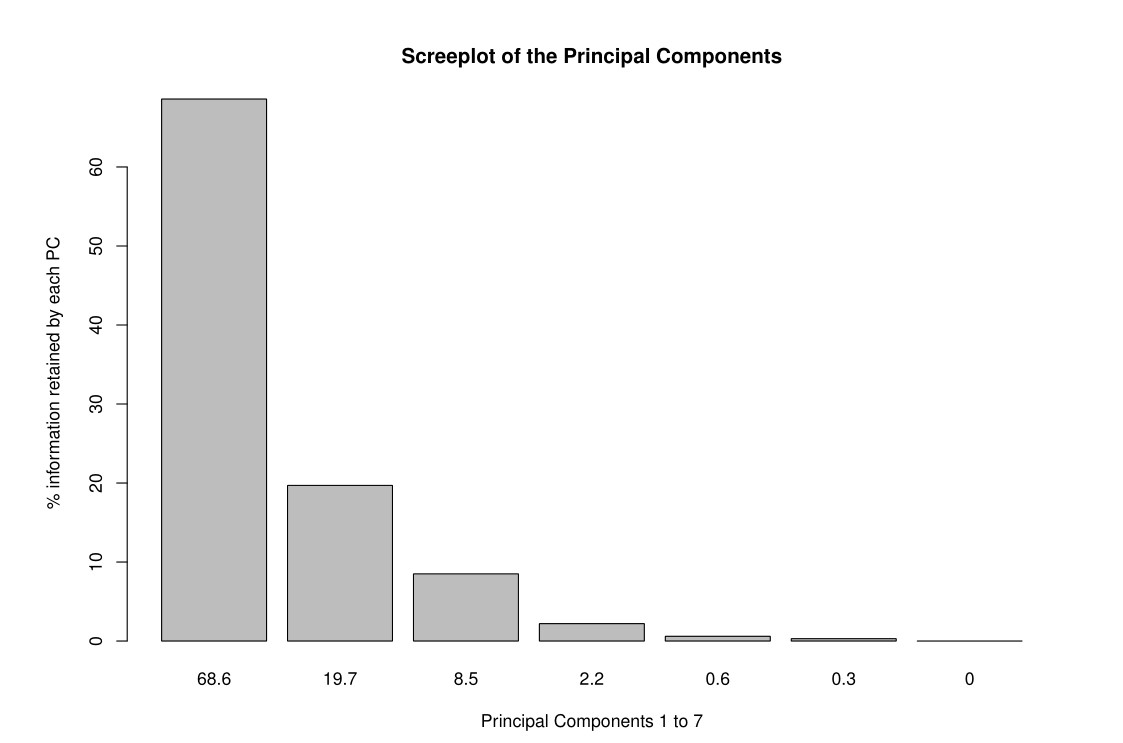
\includegraphics{./PCA screeplot.jpg}
\caption{PCA Screeplot}
\end{figure}
\end{frame}

\begin{frame}{Principal Components Analysis: Eigenvectors}
\protect\hypertarget{principal-components-analysis-eigenvectors}{}
\begin{figure}
\centering
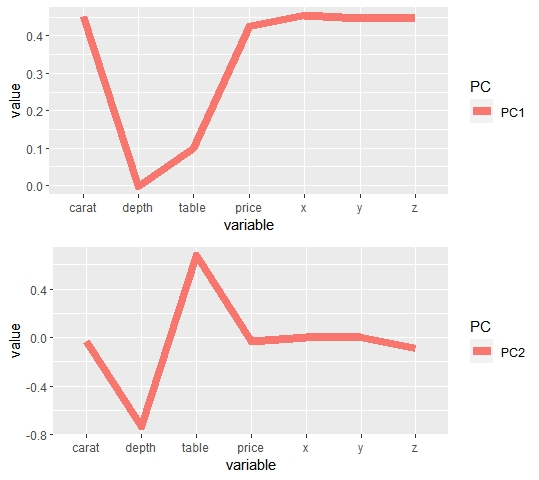
\includegraphics[width=\textwidth,height=0.85\textheight]{./Eigenvector Plot.jpeg}
\caption{Plot of EigenVectors}
\end{figure}
\end{frame}

\begin{frame}{Biplot}
\protect\hypertarget{biplot}{}
\begin{figure}
\centering
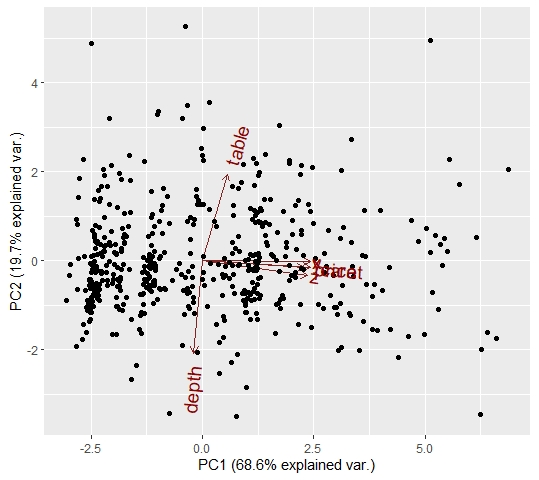
\includegraphics[width=\textwidth,height=0.85\textheight]{./Biplot PCA.jpeg}
\caption{PCA Biplot}
\end{figure}
\end{frame}

\begin{frame}{Principal Components Regression}
\protect\hypertarget{principal-components-regression}{}
\begin{itemize}
\tightlist
\item
  We conducted a Principal Components Regression with diamond price as
  the response variable\linebreak
\item
  The PCA excluding price was almost identical to the original
  PCA\linebreak
\item
  We were able to explain over 80\% of the variation in price using just
  the first two principal components as predictors\linebreak 
\item
  A more parsimonious model!\linebreak
\end{itemize}
\end{frame}

\begin{frame}{Summary of Models Predicting Diamond Price}
\protect\hypertarget{summary-of-models-predicting-diamond-price}{}
\begin{table}[ht]
\centering
\begin{tabular}{rcc}
  \hline
 Model \vline & No. of Predictors & Adjusted $R^2$ \\ 
  \hline
Full Model \vline & 9 & 0.9198\\
   \hline
Best Model \vline & 7 & 0.9198\\
\hline
Numeric Model \vline & 7 & 0.8592\\
Two PC \vline & 2 & 0.8092\\
All PC \vline & 6 & 0.8695\\
\end{tabular}
\end{table}
\end{frame}

\begin{frame}{Leading Question 2 \ldots{} and the issues we
encountered\ldots{}}
\protect\hypertarget{leading-question-2-and-the-issues-we-encountered}{}
\begin{itemize}
\tightlist
\item
  The diamonds dataset includes 280 interactions between different
  levels of the categorical variables\linebreak
\item
  Our second leading question was to investigate if we could classify
  the diamonds data more simply using analytical techniques such as LDA
  and CA\linebreak 
\end{itemize}
\end{frame}

\begin{frame}{Problems encountered}
\protect\hypertarget{problems-encountered}{}
\begin{itemize}
\item
  Despite a correlation of 0.9216, `carat' was not a great predictor of
  `price'
\item
  LDA did not work with the full dataset
\end{itemize}
\end{frame}

\begin{frame}{Linear Discriminatory Analysis}
\protect\hypertarget{linear-discriminatory-analysis}{}
\begin{figure}
\centering
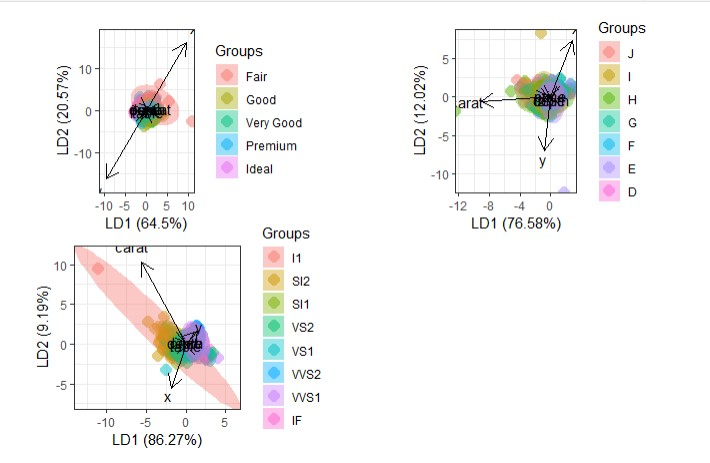
\includegraphics{./LDA ordination plots.jpg}
\caption{LDA ordination plots}
\end{figure}
\end{frame}

\begin{frame}{Slicing the dataset 1}
\protect\hypertarget{slicing-the-dataset-1}{}
\begin{figure}
\centering
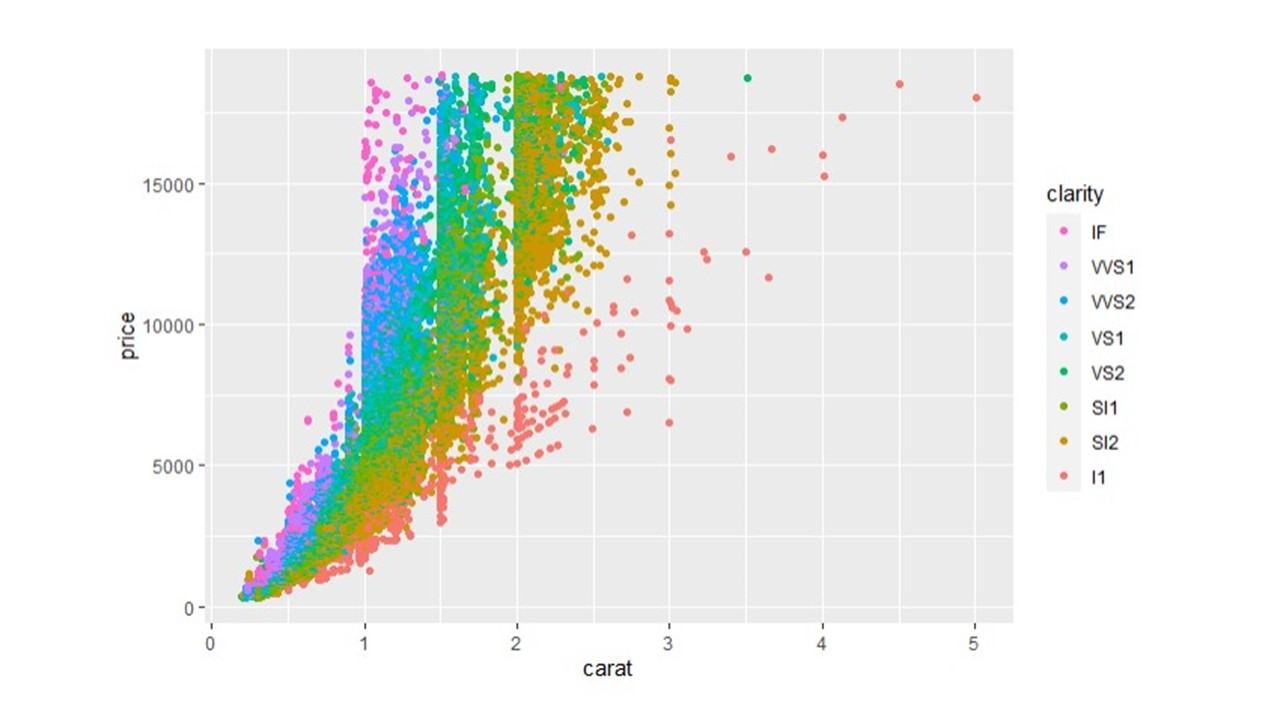
\includegraphics{./coloured scatterplot carat vs price vs clarity 2.jpg}
\caption{Carat vs Price vs Clarity}
\end{figure}
\end{frame}

\begin{frame}{Slicing the dataset 2}
\protect\hypertarget{slicing-the-dataset-2}{}
\begin{figure}
\centering
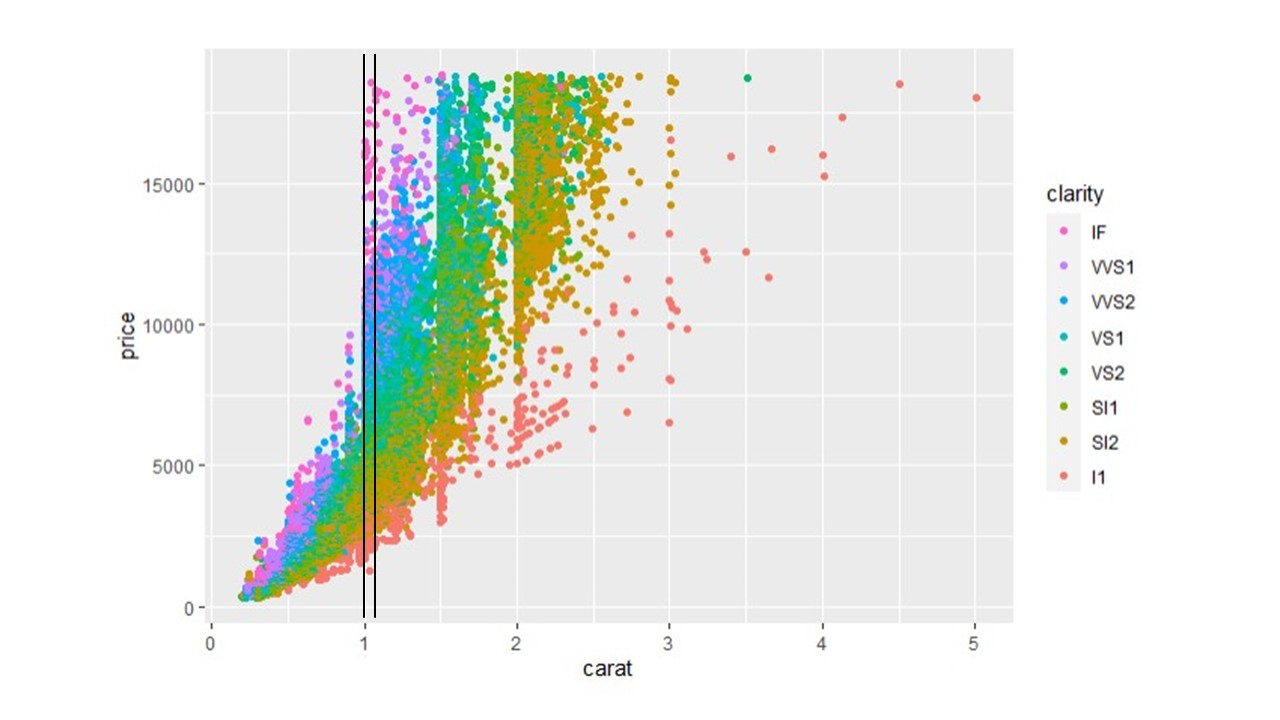
\includegraphics{./scatterplot vertical slice.jpg}
\caption{Carat vs Price vs Clarity: vertical slice}
\end{figure}
\end{frame}

\begin{frame}{Slicing the dataset 3}
\protect\hypertarget{slicing-the-dataset-3}{}
\begin{figure}
\centering
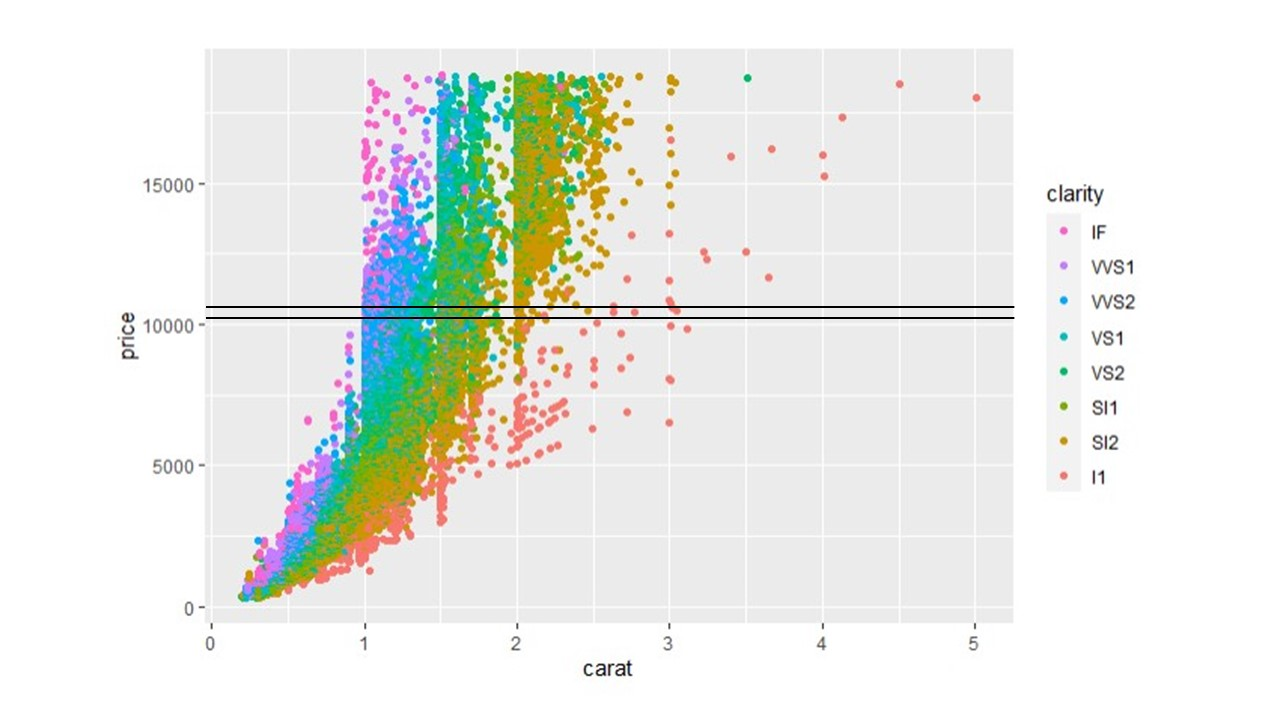
\includegraphics{./coloured scatterplot carat vs price vs clarity 3.jpg}
\caption{Carat vs Price vs Clarity: horizontal slice}
\end{figure}
\end{frame}

\begin{frame}{Slicing the dataset 4}
\protect\hypertarget{slicing-the-dataset-4}{}
\begin{figure}
\centering
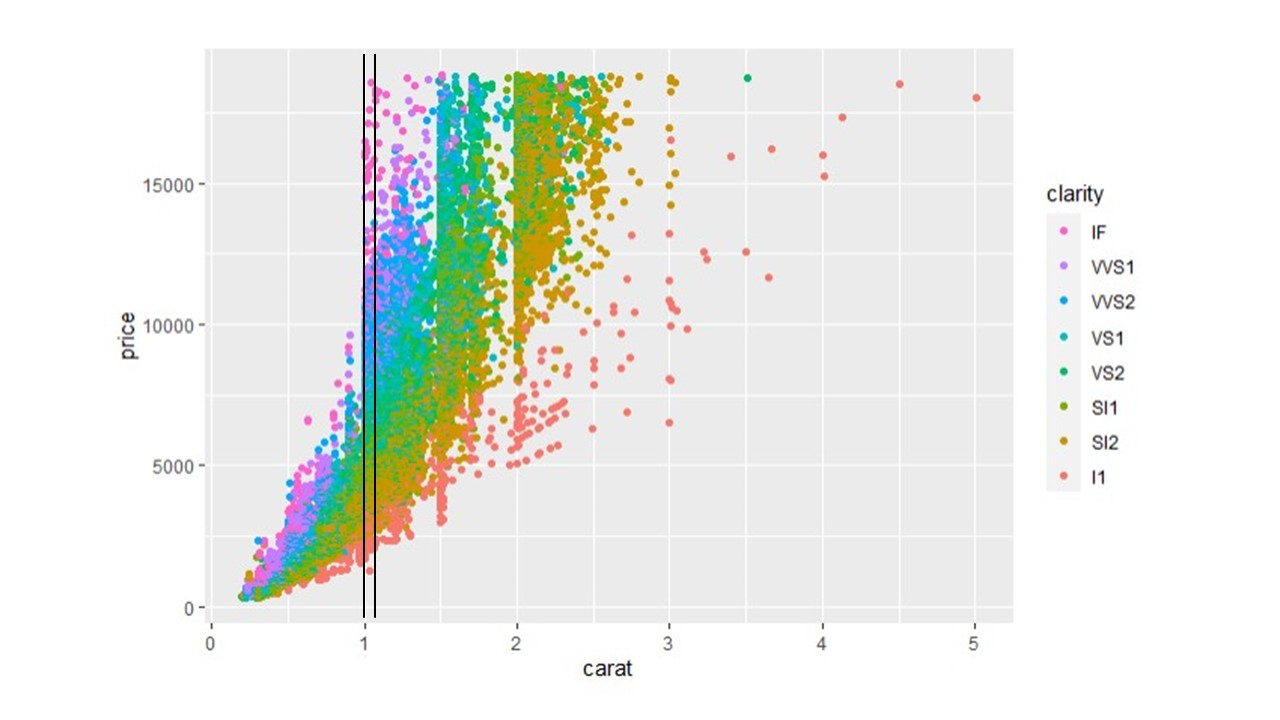
\includegraphics{./scatterplot vertical slice.jpg}
\caption{Carat vs Price vs Clarity: vertical slice}
\end{figure}
\end{frame}

\begin{frame}{Colour bands evident in sliced version}
\protect\hypertarget{colour-bands-evident-in-sliced-version}{}
\begin{figure}
\centering
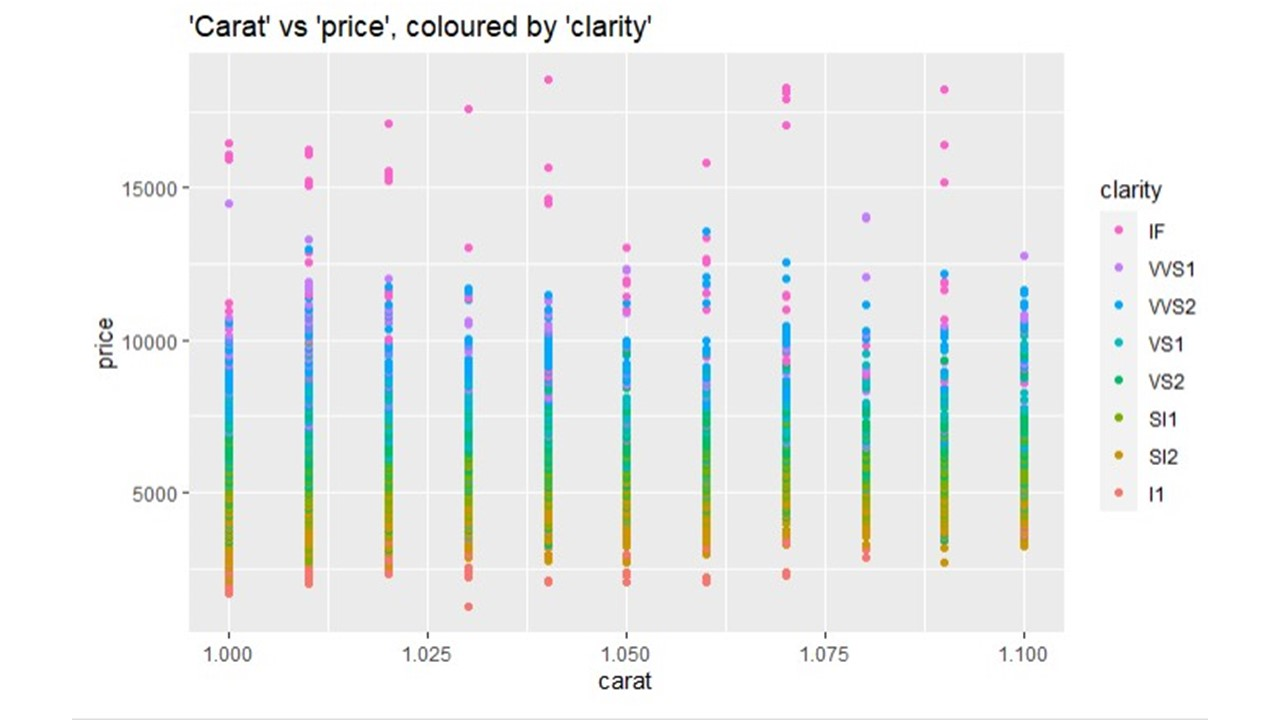
\includegraphics{./carat vs price vs clarity 2.jpg}
\caption{Carat vs Price vs Clarity: sliced 1}
\end{figure}
\end{frame}

\begin{frame}{Colour bands evident in sliced version 4}
\protect\hypertarget{colour-bands-evident-in-sliced-version-4}{}
\begin{figure}
\centering
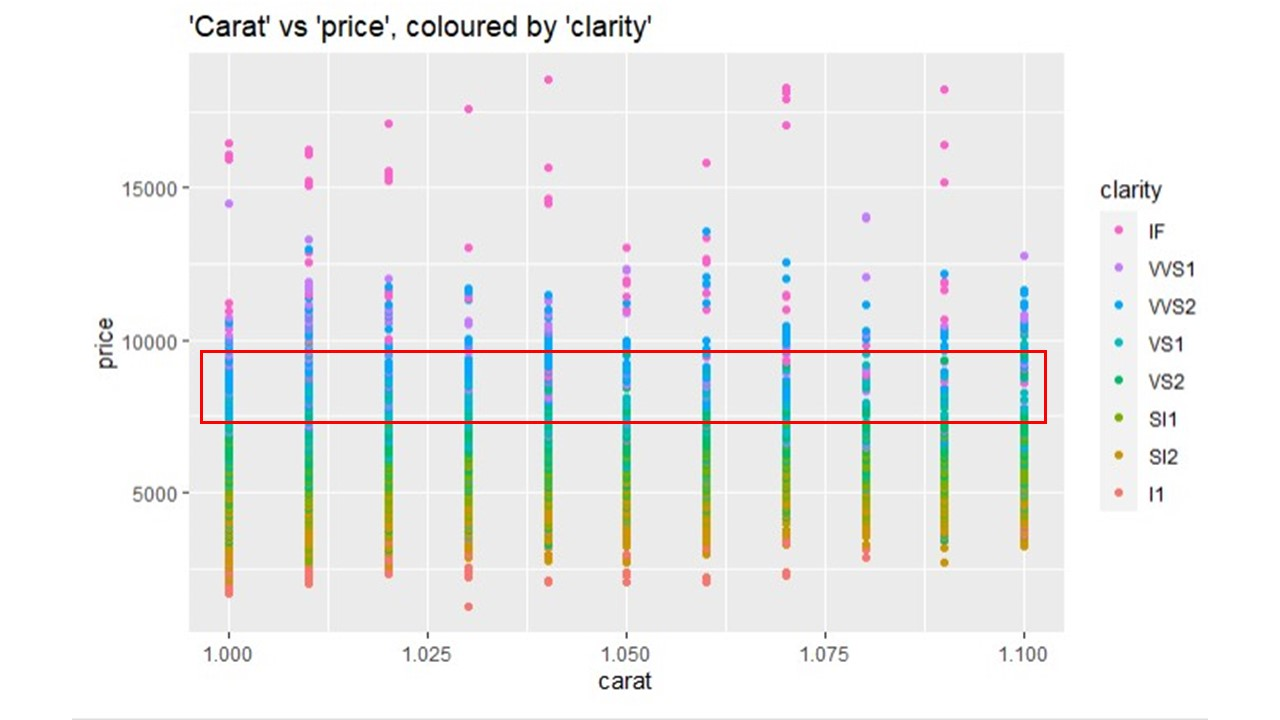
\includegraphics{./carat vs price vs clarity sliced.jpg}
\caption{Carat vs Price vs Clarity: sliced 2}
\end{figure}
\end{frame}

\end{document}
